\section{Broadcast Receivers, Push Notifications \& Services}
\subsection{Broadcast Receiver}

\begin{breakbox}
\begin{itemize}
\tightlist
\item
  Is an ``event handler'' Android component
\item
  Typically used to process an event e.g.~by starting an activity that
  interacts with the user or by starting or resuming a service for
  background work
\item
  Events include

  \begin{itemize}
  \tightlist
  \item
    System event
  \item
    App-created events
  \end{itemize}
\end{itemize}
\end{breakbox}

\begin{breakbox}
\boxtitle{Registration}

\begin{itemize}
\tightlist
\item
  Via the Android Manifest
\item
  Dynamically via the context
\end{itemize}
\end{breakbox}

\begin{breakbox}
\boxtitle{Implementation}

The receiver needs to extend the class BroadcastReceiver and with
it the method onReceive().

\end{breakbox}

\begin{breakbox}
\boxtitle{Examples for Broadcasts}

\begin{enumerate}
\item
  android.app.action.\\
  ACTION\_PASSWORD\_SUCCEEDED
\item
  android.bluetooth.adapter.action.\\
  DISCOVERY\_STARTED
\item
  android.intent.action.\\
  ACTION\_AIRPLANE\_MODE\_CHANGED
\item
  android.intent.action.BATTERY\_LOW
\item
  android.net.wifi.\\
  SCAN\_RESULTS\_AVAILABLE\_ACTION
\end{enumerate}
\end{breakbox}

\subsection{Push notifications}

\begin{breakbox}
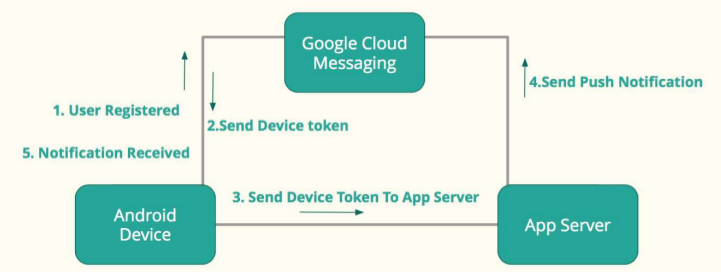
\includegraphics[width=0.24\textwidth]{figures/pushNotificationFlow.png}
\end{breakbox}

\begin{breakbox}
\boxtitle{Implementation}

\begin{lstlisting}
public class MyMessageReceivedInstance extends FirebaseMessagingService {
    public void onMessageReceived(RemoteMessage remoteMessage) {
        Intent intent=new Intent(this,MainActivity.class);
        ...
        notificationBuilder.setContentText(remoteMessage.getNotification().getBody());
        ...
        notificationManager.notify(0,notificationBuilder.build());
    }
}
\end{lstlisting}
\end{breakbox}


\subsection{Services}

\begin{breakbox}
\begin{itemize}
\tightlist
\item
  Are components that perform long-lasting operations in the background
  even when the user is not interacting with the application
\item
  They have their own lifecycle
\item
  Typically start one or more threads to perform work outside the UI
  tread
\end{itemize}
\end{breakbox}

\begin{breakbox}
\boxtitle{Different forms of services}

\begin{itemize}
\tightlist
\item
  Started services

  \begin{itemize}
  \tightlist
  \item
    Invoked with startService(Intent,..)
  \item
    Stopped when stopSelf()or stopService()is called
  \end{itemize}
\item
  Bound services

  \begin{itemize}
  \tightlist
  \item
    Binding is done with bindService()
  \item
    Allows for interprocess communication to send requests, get results,
    etc.
  \item
    Stopped when no other component is bound to it
  \end{itemize}
\end{itemize}

\end{breakbox}

\begin{breakbox}
\boxtitle{Start / Stop}

\begin{itemize}
\tightlist
\item
  Unlike the activity lifecycle callback methods, you are not required
  to call the superclass implementation of the service lifecycle methods
\item
  When handling multiple concurrent requests you may use
  stopSelf(startID) with the startID from onStartCommand()
\item
  Please always stop services to avoid wasting resources and consuming
  battery power
\end{itemize}

\end{breakbox}

